
\subsubsection{Solución}
 
\textbf{Solución analítica del circuito:}

Empezamos por la sustitución de los valores dados en el ejercicio, donde $\frac{R}{L}=1$ y $\frac{1}{LC}=5$. Con esto podemos reescribir nuestra ecuación de la siguiente forma:

\begin{equation}
	\frac{d^2V_c(t)}{dt^2}+\frac{dV_c(t)}{dt}+5V_g(t)=5V_g(t)
\end{equation}

\noindent Realizamos la sustitución de $V_c(t)=y(t)$ y $V_g(t)=x(t)$

\begin{equation}
	\frac{d^2y(t)}{dt^2}+\frac{dy(t)}{dt}+5y(t)=5x(t)
\end{equation}

\noindent Con dichos cambios ya podemos empezar a aplicar la transformada de Laplace a ambos lados de la ecuación

\begin{equation}
	\Laplace\{{\frac{d^2y(t)}{dt^2}+\frac{dy(t)}{dt}+5y(t)}\}=\Laplace\{{5x(t)}\}
\end{equation}

\begin{equation}
	s^2Y(s)+sY(s)+5Y(s)=5X(s)
\end{equation}

\noindent Factorizamos $Y(s)$ y $X(s)$

\begin{equation}
	Y(s)(s^2+s+5)=5X(s)
\end{equation}

\noindent Si reacomodamos la expresión finalmente llegamos a la función de transferencia

\begin{equation}
	H(s)=\frac{Y(s)}{X(s)}=\frac{5}{(s^2+s+5)}
\end{equation}

\noindent Si consideramos la entrada un escalón, es decir que $X(s)=1$ simplificamos la expresión a 

\begin{equation}
	Y(s)=\frac{5}{(s^2+s+5)}
\end{equation}

\noindent Una vez teniendo la transformada de Laplace podemos aplicar la antitransformada para llegar a la ecuación solución del sistema.

\begin{equation}
	\Laplace^-1\{Y(s)\}=\Laplace^-1\{\frac{5}{(s^2+s+5)}\}
\end{equation}

\begin{equation}
	y(t)=\frac{10\sqrt(19)e^\frac{-t}{2}sin(\frac{\sqrt(19)t)}{2})}{19}
\end{equation}

\noindent\textbf{Representación grafica: }



\begin{figure}[H]
	\centering
	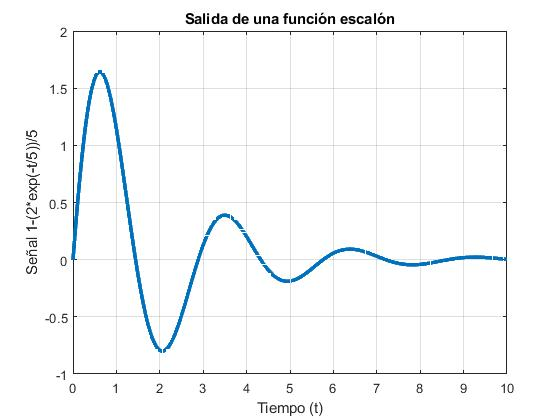
\includegraphics[width=0.7\linewidth]{salidaejercicio1}
	\caption{Gráfica de la función muestreada}
	\label{fig:salidaejercicio1}
\end{figure}
